\section{Results}
\label{sec:Results}

This section presents the main results obtained in this research, as well as their detailed analysis is performed.

\subsection{Subsection name}
\label{sec:}

\begin{table*}[!h]
\caption{An example of a simple table containing descriptive statistics.}
\label{tab:tab_descr_1}
\setlength{\arrayrulewidth}{1.05 pt}
\renewcommand{\arraystretch}{1.1}
\begin{tabular*}{1.0\textwidth}{@{\extracolsep{\fill}}lrr}
\hline
Parameter & Column Name & Column Name \\
\hline
Mean, $\mu$ & 0.79 & 0.98 \\
\hline
\end{tabular*}
\begin{spacing}{0.5}
{\scriptsize Note: There are explanations to the table.}
\end{spacing}
\end{table*}

\subsection{Subsection name}
\label{sec:}

\begin{table*}[!h]
\caption{An example of more complicated table containing estimates of the model parameters.}
\label{tab:}
\setlength{\arrayrulewidth}{1.05 pt}
\renewcommand{\arraystretch}{1.1}
\begin{tabular*}{1.0\textwidth}{@{\extracolsep{\fill}}lrrr}
\hline
Parameter & \textit{Column Name} & \textit{Column Name} & \textit{Column Name} \\
\hline

\multicolumn{4}{l}{\textit{Group Name}} \\
$\mu$ & 0.30\textsuperscript{***} {\footnotesize (0.01)} & 0.30\textsuperscript{***} {\footnotesize (0.01)} & 0.30\textsuperscript{***} {\footnotesize (0.01)} \\
$\phi$ & 0.30\textsuperscript{***} {\footnotesize (0.01)} & 0.30\textsuperscript{***} {\footnotesize (0.01)} & 0.30\textsuperscript{***} {\footnotesize (0.01)} \\

\multicolumn{4}{l}{\textit{Group Name}} \\
$\mu$ & 0.40\textsuperscript{*} {\footnotesize (0.17)} & 0.40\textsuperscript{*} {\footnotesize (0.17)} & 0.40\textsuperscript{*} {\footnotesize (0.17)} \\
$\phi$ & 0.40\textsuperscript{*} {\footnotesize (0.17)} & 0.40\textsuperscript{*} {\footnotesize (0.17)} & 0.40\textsuperscript{*} {\footnotesize (0.17)} \\

\hline
\end{tabular*}
\begin{spacing}{0.5}
{\scriptsize Note: Standard errors of coefficients are given in parentheses. The levels of significance notation: *** -- 1\%, ** -- 5\%, * -- 10\%.}
\end{spacing}
\end{table*}

\subsection{Subsection name}
\label{sec:}

\begin{figure*}[!h]
\centering
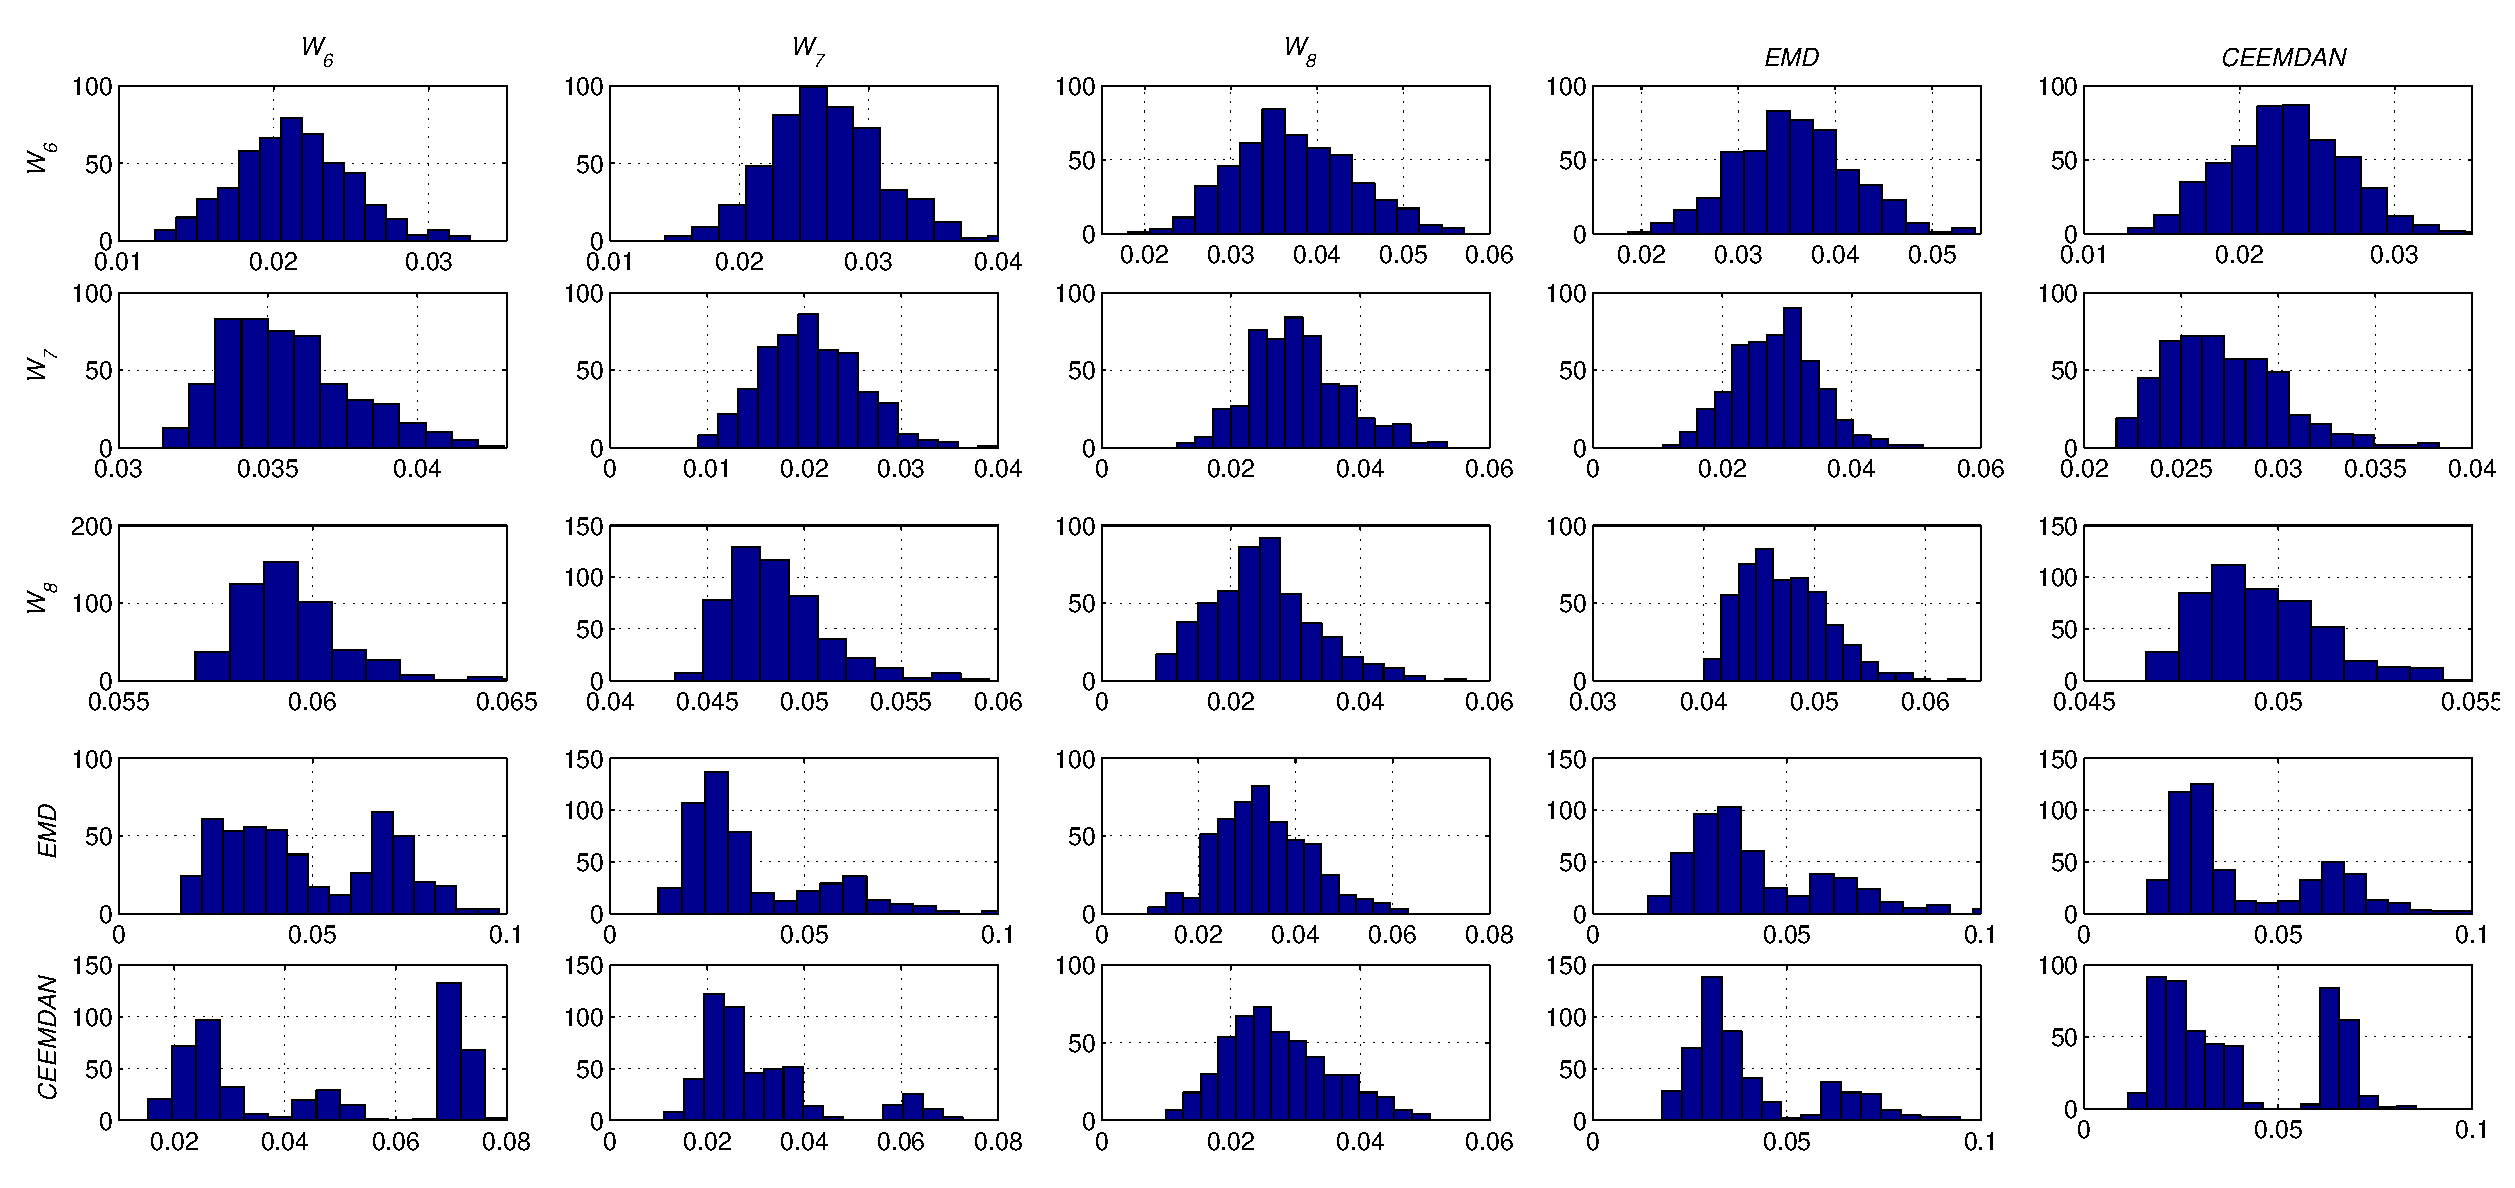
\includegraphics[width=1.0\textwidth,keepaspectratio]{Figure}
\caption{Figure Title.}
\label{fig:}
\end{figure*}